% Unofficial CU Boulder Research Poster Template
% Modified by Ashish Srivastava, 2022/11/18 for Senior Thesis
% a fork of https://github.com/anishathalye/gemini

\documentclass[final]{beamer}

% ====================
% Packages
% ====================

\usepackage[T1]{fontenc}
\usepackage{lmodern}
\usepackage[size=custom,width=120,height=90,scale=1.0]{beamerposter}
\usetheme{gemini}
\usecolortheme{cuboulder}
\usepackage{graphicx}
\usepackage{booktabs}
\usepackage{doi}
\usepackage[numbers]{natbib}
\usepackage[patch=none]{microtype}
\usepackage{tikz}
\usetikzlibrary{arrows.meta}
\usepackage{pgfplots}
\pgfplotsset{compat=1.18}
\usepackage{anyfontsize}
% \usepackage{algorithmic}
% \usepackage{algpseudocode}
% \usepackage{algorithm2e}
\usepackage{subfig}

\pdfstringdefDisableCommands{%
\def\translate#1{#1}%
}

% ====================
% Lengths
% ====================

% If you have N columns, choose \sepwidth and \colwidth such that
% (N+1)*\sepwidth + N*\colwidth = \paperwidth
\newlength{\sepwidth}
\newlength{\colwidth}
\setlength{\sepwidth}{0.025\paperwidth}
\setlength{\colwidth}{0.3\paperwidth}

\newcommand{\separatorcolumn}{\begin{column}{\sepwidth}\end{column}}

% ====================
% Title
% ====================

\title{Experimental and Computational Analyses of \\ Droplet Motion in Straight, Rectangular Microchannels}

\author{\underline{Ashish Srivastava} \inst{1} \and Gesse A. Roure \inst{1} \and Robert H. Davis \inst{1}}


\institute[shortinst]{\inst{1} University of Colorado, Boulder} % \samelineand \inst{2} Another Institute}


% ====================
% Footer (optional)
% ====================

\footercontent{
  \href{https://www.colorado.edu/chbe/}{https://www.colorado.edu/chbe/} \hfill
  JSCBB, 3415 Colorado Ave, Boulder, CO --- 80303 \hfill
  \href{mailto:ashish.srivastava@colorado.edu}{ashish.srivastava@colorado.edu}}
% (can be left out to remove footer)

% ====================
% Logo (optional)
% ====================

% use this to include logos on the left and/or right side of the header:
% \logoright{\includegraphics[height=7cm]{logo1.pdf}}
% \logoleft{\includegraphics[height=7cm]{logo2.pdf}}

% ====================
% Body
% ====================

\begin{document}
\addtobeamertemplate{headline}{}
{
    \begin{tikzpicture}[remember picture,overlay]
      \node [anchor=north west, inner sep=3cm] at ([xshift=0.0cm,yshift=1.5cm]current page.north west)
      {
\includegraphics[height=6.0cm]{logos/ChemBioEng_rev_bw_left.png}}; 
      \node [anchor=north east, inner sep=3cm] at ([xshift=0.0cm,yshift=2.75cm]current page.north east)
      {
\includegraphics[height=9.0cm]{logos/CU-seal.png}};
    \end{tikzpicture}
}

\begin{frame}[t]
\begin{columns}[t]
\separatorcolumn

\begin{column}{\colwidth}

  \begin{block}{Introduction}

    \begin{itemize}
        \item Microfluidics can be leveraged for applications such as drug delivery, single-cell assays, ``lab-on-a-chip"/$\mu$TAS (micrometer-scale total analysis system)
        \item Low Reynolds number regime (viscous dissipation $\gg$ inertial effects)
        \item \textbf{Objective:} quantify the steady-state velocity and deformation of droplets as a result of changing different parameters of the flow
        \begin{itemize}
            \item Boundary-integral simulations
            \item Macroscopic flow cell and computer vision code
        \end{itemize}

    \end{itemize}
    \begin{align*}
        Re = \frac{\rho UH}{\mu_e} = \frac{\text{inertial forces}}{\text{viscous forces}} \ll 1
    \end{align*}

  \end{block}

  \begin{block}{Numerical Methods: Boundary-Integral Method with Moving Frame}
    \begin{itemize}
        \item Numerical solution of the Boundary-Integral form of the Stokes equations
        \begin{itemize}
            \item  $\boldsymbol{u(\boldsymbol{y}}) \equiv$ velocity on drop surface
            \item $\boldsymbol{q}(\boldsymbol{y}) \equiv$ density function on domain surface
        \end{itemize}
        \item Only requires meshing of the interfaces (drop + channel)
        \item A moving frame is used to further reduce computational load
        \item For straight channels, the undisturbed flow is given by Boussinesq's solution
    \end{itemize}   
    \begin{columns}
        \small
        \begin{column}{.45\textwidth} % Left column and width

        \resizebox{\linewidth}{!}{
            \begin{minipage}{\linewidth}
                \vspace*{1cm}
                
                \begin{align*} % Integral form of Stokes u equation
                    \boldsymbol{u}(\boldsymbol{y}) &= \frac{2}{\lambda+1}\left[\boldsymbol{u}_{\infty}(\boldsymbol{y})+\boldsymbol{F}(\boldsymbol{y})+2 \int_{S_{\infty}} \boldsymbol{q}(\boldsymbol{x}) \cdot \boldsymbol{\tau}(\boldsymbol{x}-\boldsymbol{y}) \cdot \boldsymbol{n}(\boldsymbol{x}) d S_x\right] \\ 
                    & +\frac{2(\lambda-1)}{\lambda+1} \int_{S_d} \boldsymbol{u}(\boldsymbol{x}) \cdot \boldsymbol{\tau}(\boldsymbol{x}-\boldsymbol{y}) \cdot \boldsymbol{n}(\boldsymbol{y}) d S_x
                    \caption{Velocity on drop surface}
                \end{align*}

                \begin{align*} % Integral form of Stokes q equation
                    \boldsymbol{q}(\boldsymbol{y}) &= -\boldsymbol{F}(\boldsymbol{y})-(\lambda-1) \int_{S_d} \boldsymbol{u}(\boldsymbol{x}) \cdot \boldsymbol{\tau}(\boldsymbol{x}-\boldsymbol{y}) \cdot \boldsymbol{n}(\boldsymbol{x}) d S_x \\
                    & -2 \int_{S_{\infty}} \boldsymbol{q}(\boldsymbol{x}) \cdot \boldsymbol{\tau}(\boldsymbol{x}-\boldsymbol{y}) \cdot \boldsymbol{n}(\boldsymbol{x}) d S_x-\frac{\boldsymbol{n}(\boldsymbol{y})}{S_{\infty}} \int_{S_{\infty}} \boldsymbol{q}(\boldsymbol{x}) \cdot \boldsymbol{n}(\boldsymbol{x}) d S_x 
                \end{align*}
                
            \end{minipage}
        }
        
        \begin{figure}
            \centering
            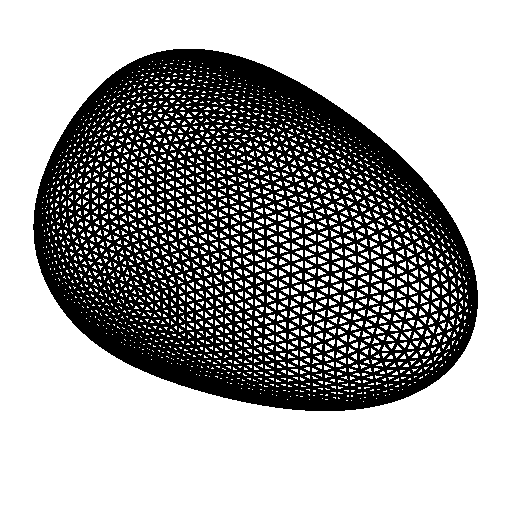
\includegraphics[width=0.45\linewidth]{figures/mesh.pdf}
            \caption{Drop mesh used for discretization}
        \end{figure}

        \end{column}

        \begin{column}{.55 \textwidth} % Right column and width

        \begin{figure}
            \centering
            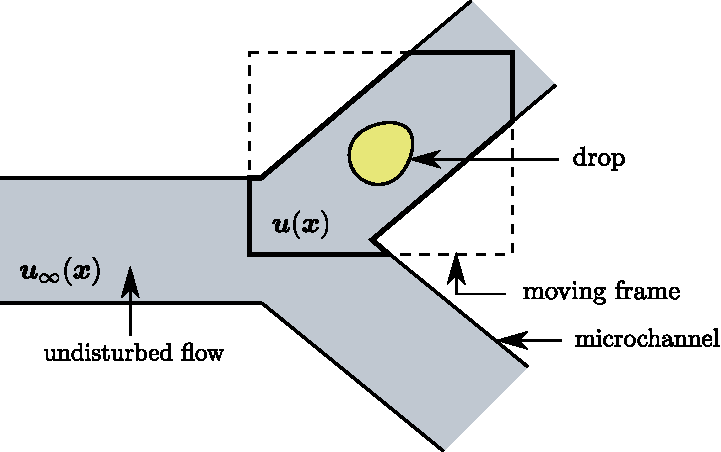
\includegraphics[width=0.98\linewidth]{figures/movingframe.pdf}
            \caption{Moving-frame approach for the solution \cite*{navarro_boundary-integral_2020, Roure_2022} }
            \label{fig:movingframe}
        \end{figure}

        \centering

        \end{column}
        \normalsize
    \end{columns}
  \end{block}

    \begin{block}{Results: Simulated Droplet Motion and Deformation}
        \begin{columns}
          \begin{column}{.66\textwidth} % Left column and width
                \vspace{1cm}
                \begin{figure}
                    \centering
                    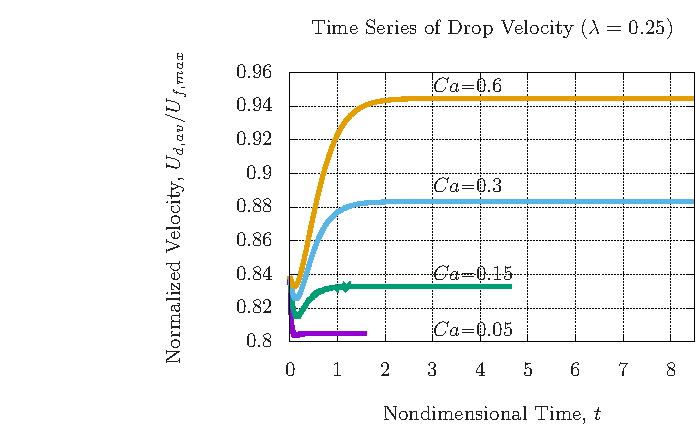
\includegraphics[width=0.9\linewidth]{figures/varyingCa.eps}
                    % \caption{Varying $Ca$, keeping $\lambda$ constant}
                \end{figure}

                \begin{figure}
                  \centering
                  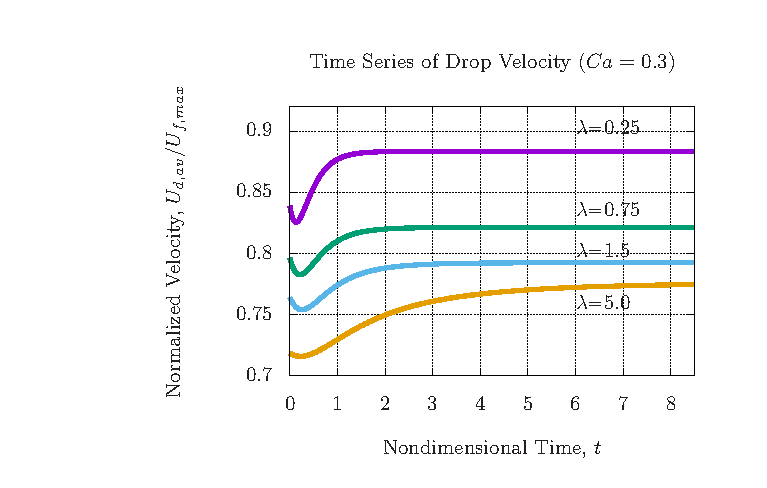
\includegraphics[width=\linewidth]{figures/varyingRMU.eps}
                  % \caption{Varying $\lambda$, keeping $\Ca$ constant}
                \end{figure}
            
          \end{column}%
          \hfill%
          \begin{column}{.34 \textwidth} % Right column and width
                \vspace{-1.5cm}
                % Ca
                \begin{align*}
                    \centering
                    Ca = \frac{\mu_e U}{\sigma} = \frac{\text{viscous forces}}{\text{surface forces}}
                \end{align*}
                \vspace{0.5cm}
                \begin{itemize}
                    \item As $Ca \nearrow$, more $t$ to reach steady state
                    \item As $Ca \nearrow$, higher steady state velocity
                    \item As $Ca \nearrow$, more deformation $\Rightarrow$ more hydrodynamic shape
                \end{itemize}

                \vspace{3cm}
                % RMU
                \begin{align*}
                    \centering
                    \lambda = \frac{\mu_d}{\mu_e} = \frac{\text{droplet viscosity}}{\text{fluid viscosity}}
                \end{align*}
                \vspace{0.5cm}
                \begin{itemize}
                    \item As $\lambda \nearrow$, more $t$ to reach steady state
                    \item As $\lambda \nearrow$, lower steady state velocity
                    \item As $\lambda \nearrow$, more deformation
                \end{itemize}
                

          \end{column}
        \end{columns}
        
    \end{block}

\end{column}

\separatorcolumn

\begin{column}{\colwidth}

  \begin{block}{Methods: Macroscopic Flow Cell}
    \begin{itemize}
        \item Droplet is introduced manually via a syringe. A syringe pump is used for the bulk fluid.
        \item Castor oil is used as the bulk fluid
        \item Droplets are made of PDMS or a Water + Glycerol mixture and then dyed
    \end{itemize}
    
    \begin{figure}
      \centering
      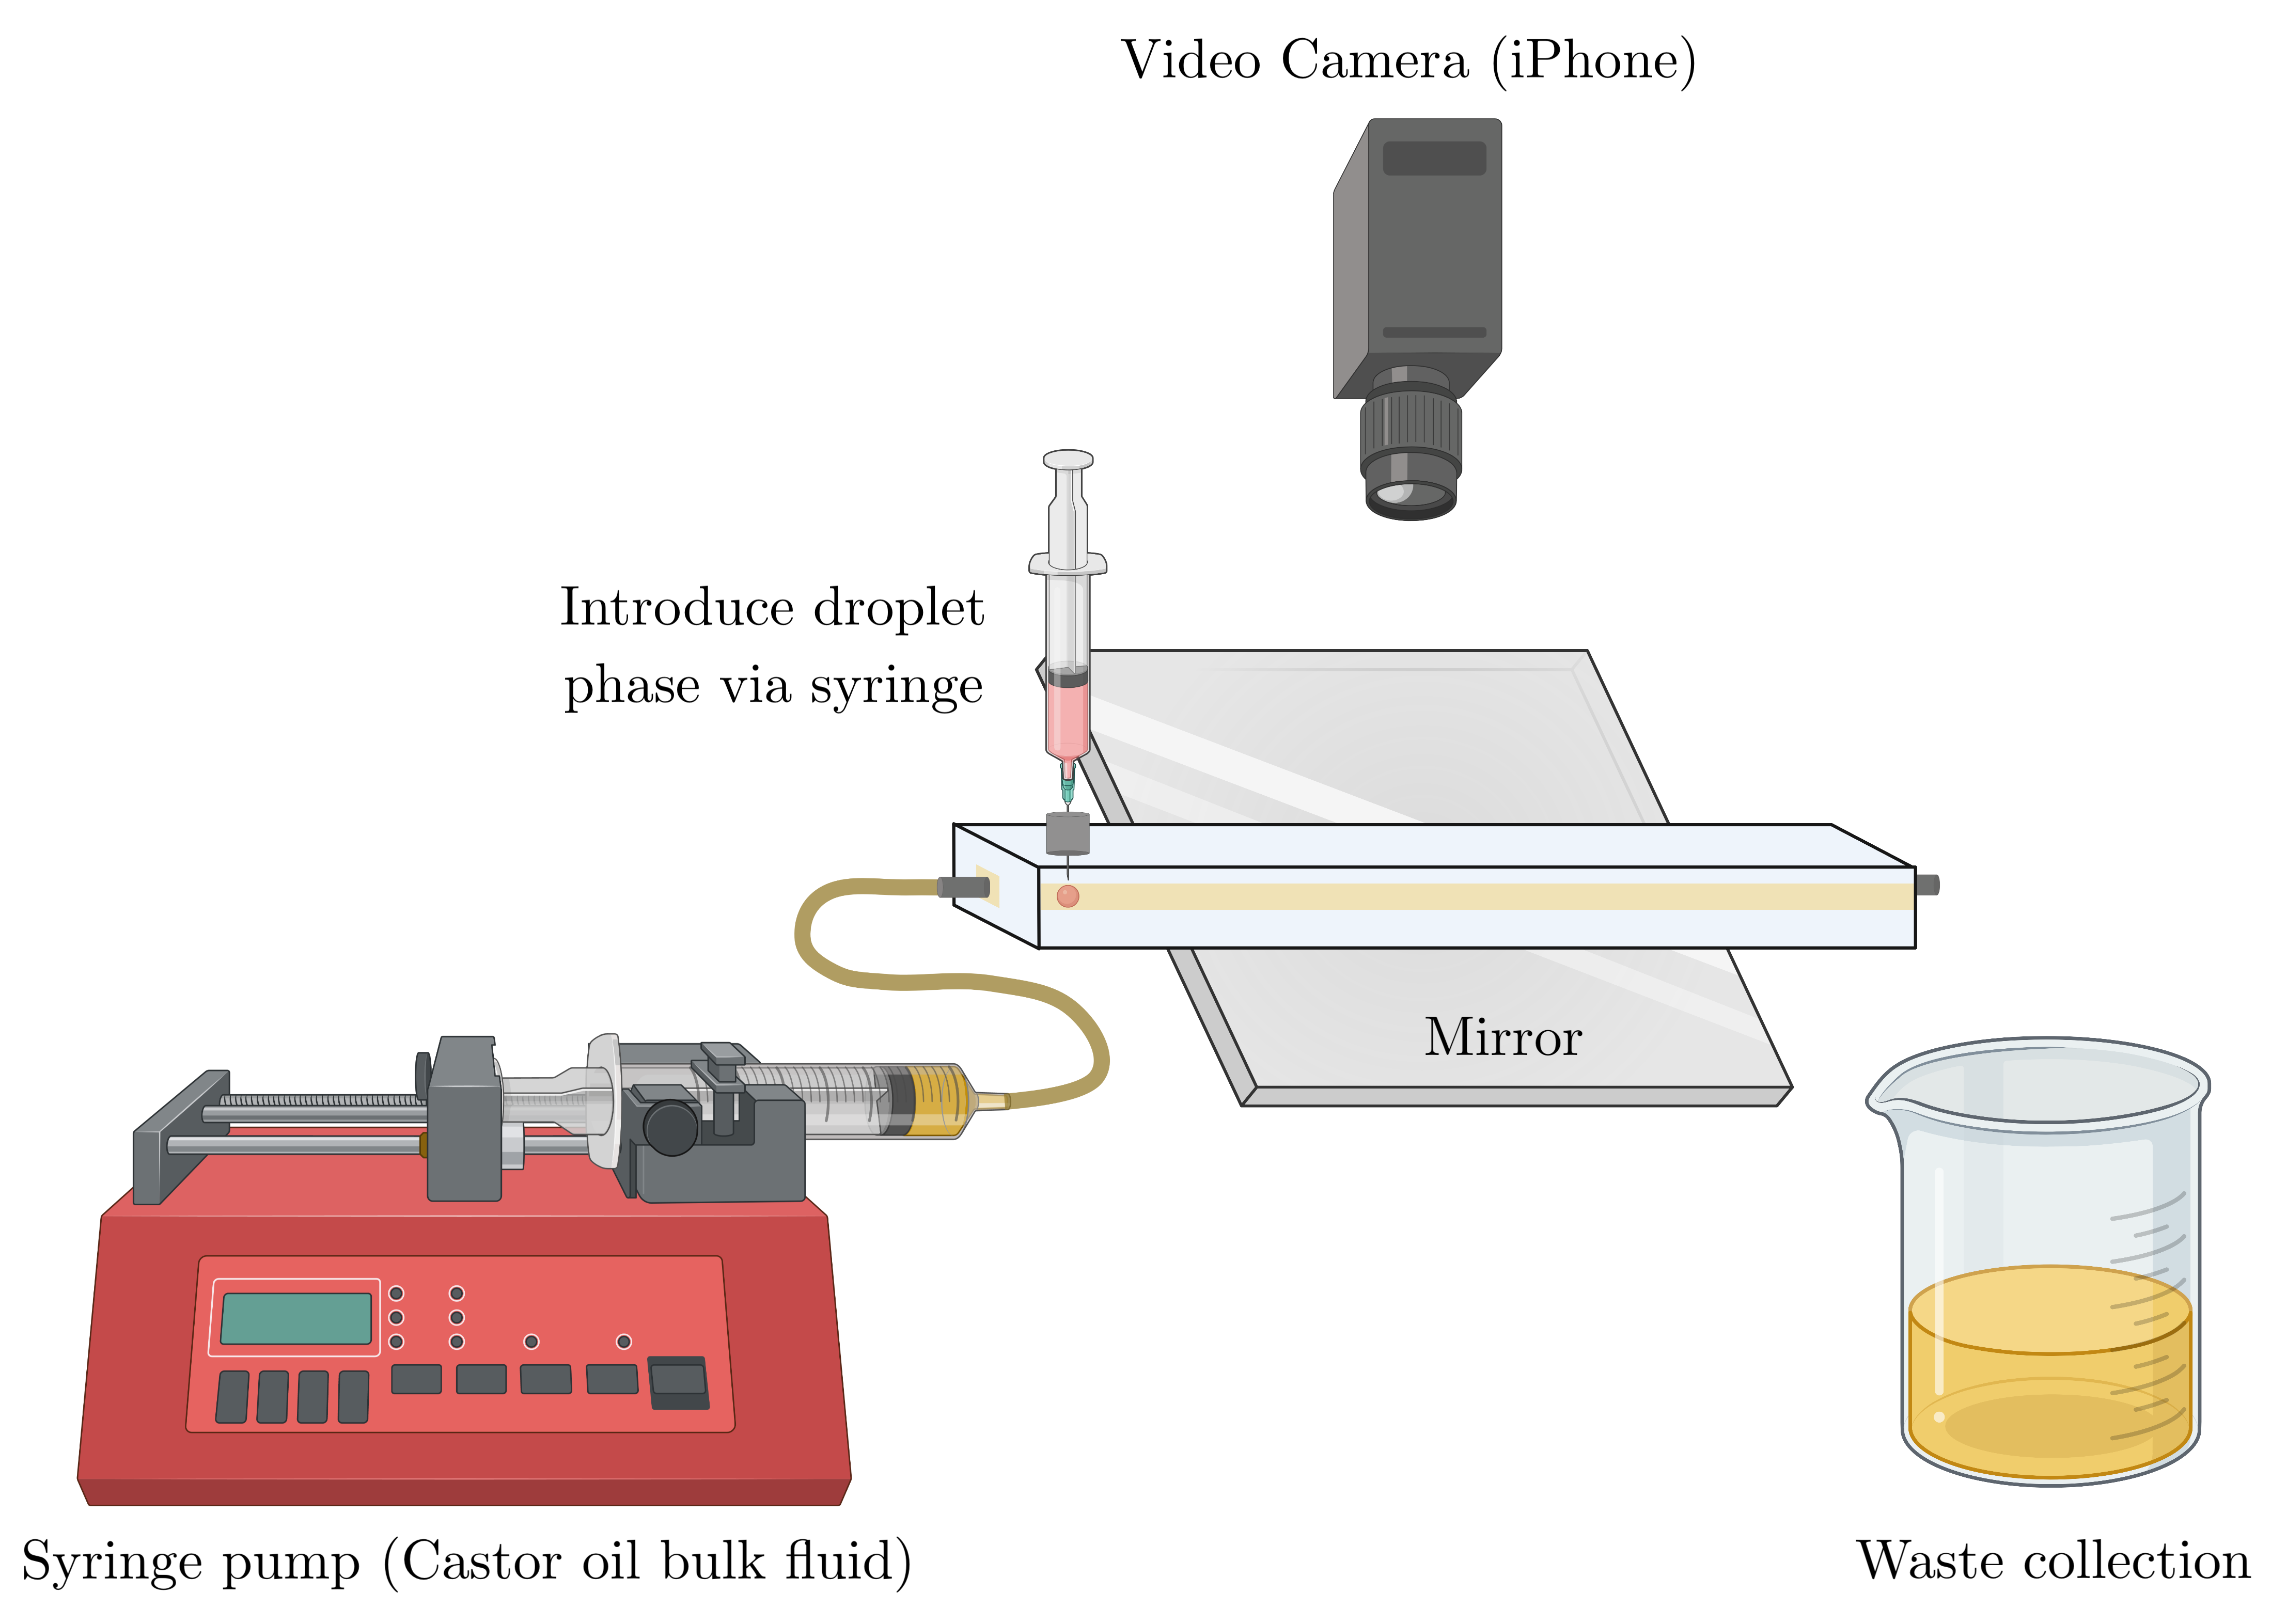
\includegraphics[width=0.6\linewidth]{figures/Flow Cell.png}
      \caption{Diagram of experimental apparatus (created with BioRender.com)}
    \end{figure}

  \end{block}

  \begin{block}{Computer Vision Algorithm}

    \begin{figure}[htbp]
        \centering
        \begin{minipage}{0.45\textwidth}
            \centering
            \subfloat[]{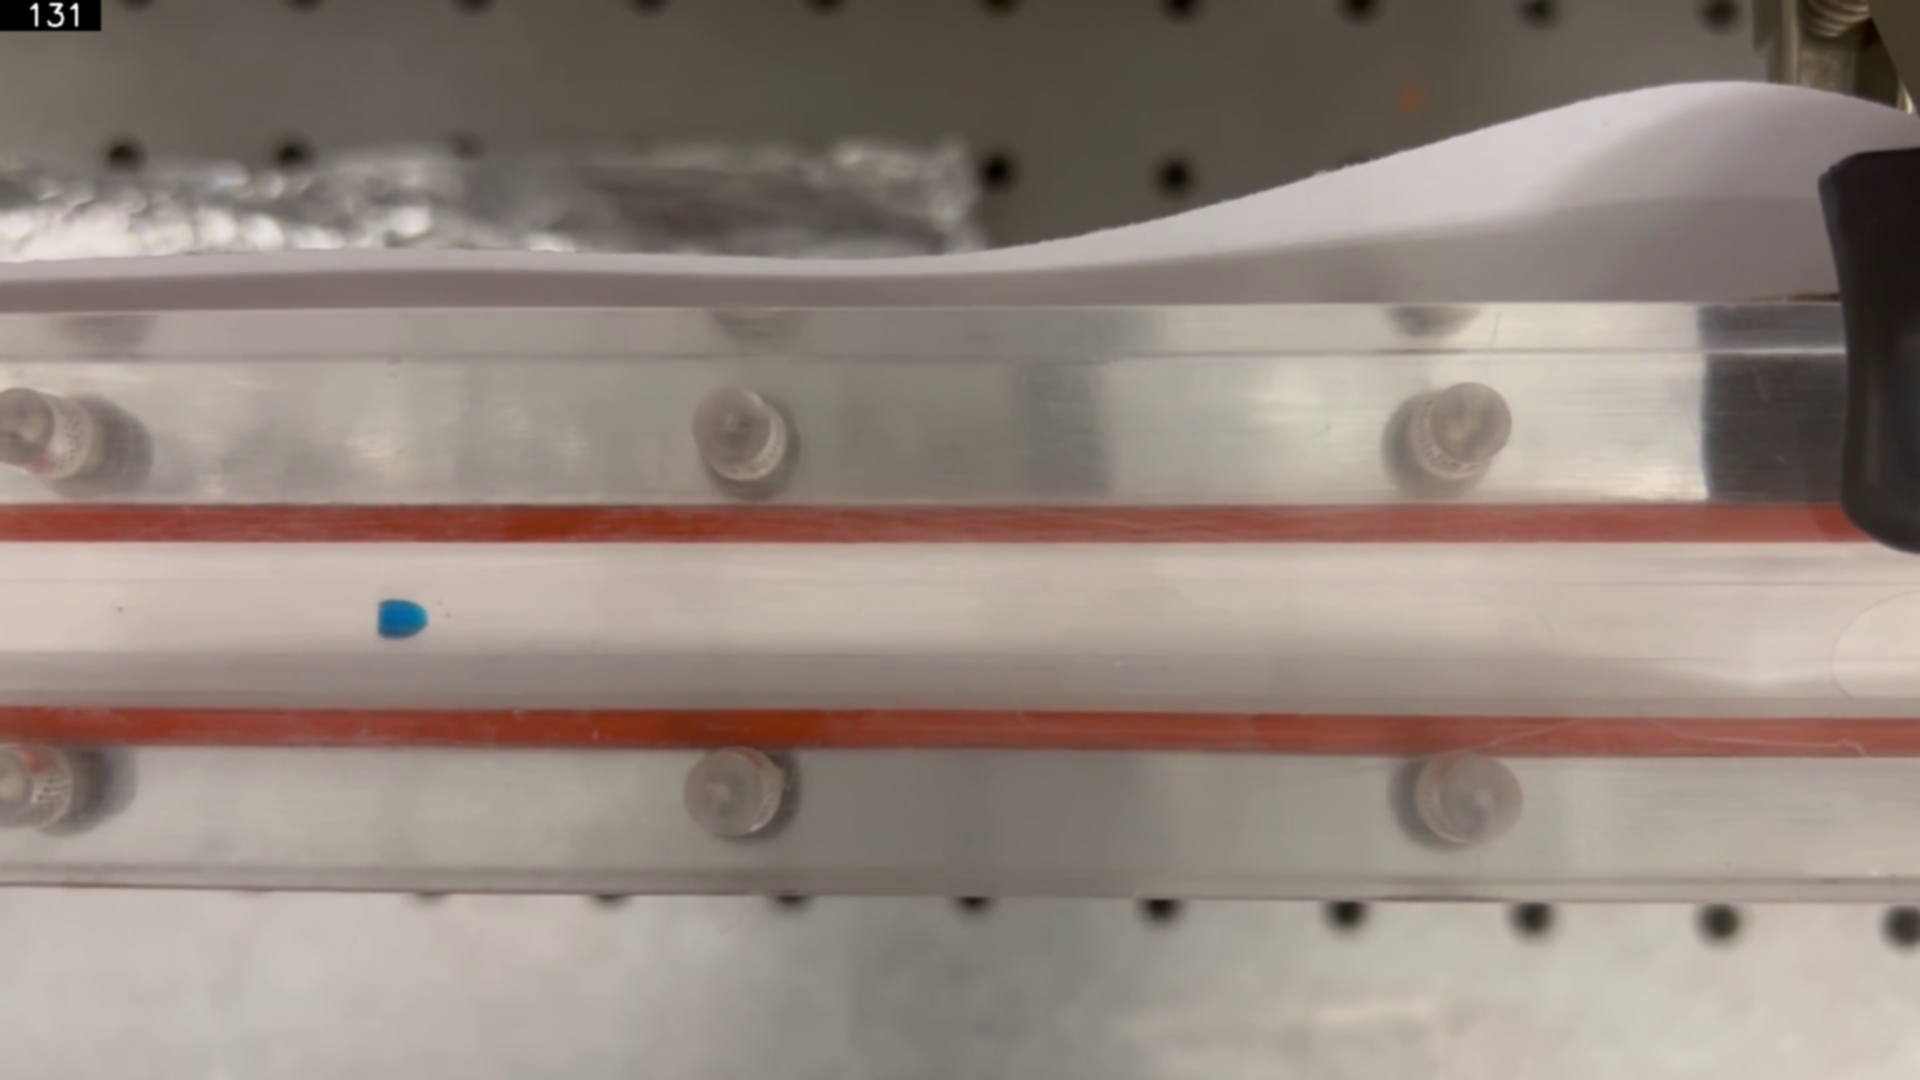
\includegraphics[width=\textwidth]{figures/frames/original_131.png}}
        \end{minipage}
        \hfill
        \begin{minipage}{0.45\textwidth}
            \begin{itemize}
            \item Used to calculate drop position and deformation
            \item Droplet center is calculated as a contour average
            \item Image correction is necessary to account for lens distortion \cite*{zhang_flexible_2000}
            \end{itemize}
        \end{minipage}
        \\
        \begin{minipage}{0.45\textwidth}
            \centering
            \subfloat[]{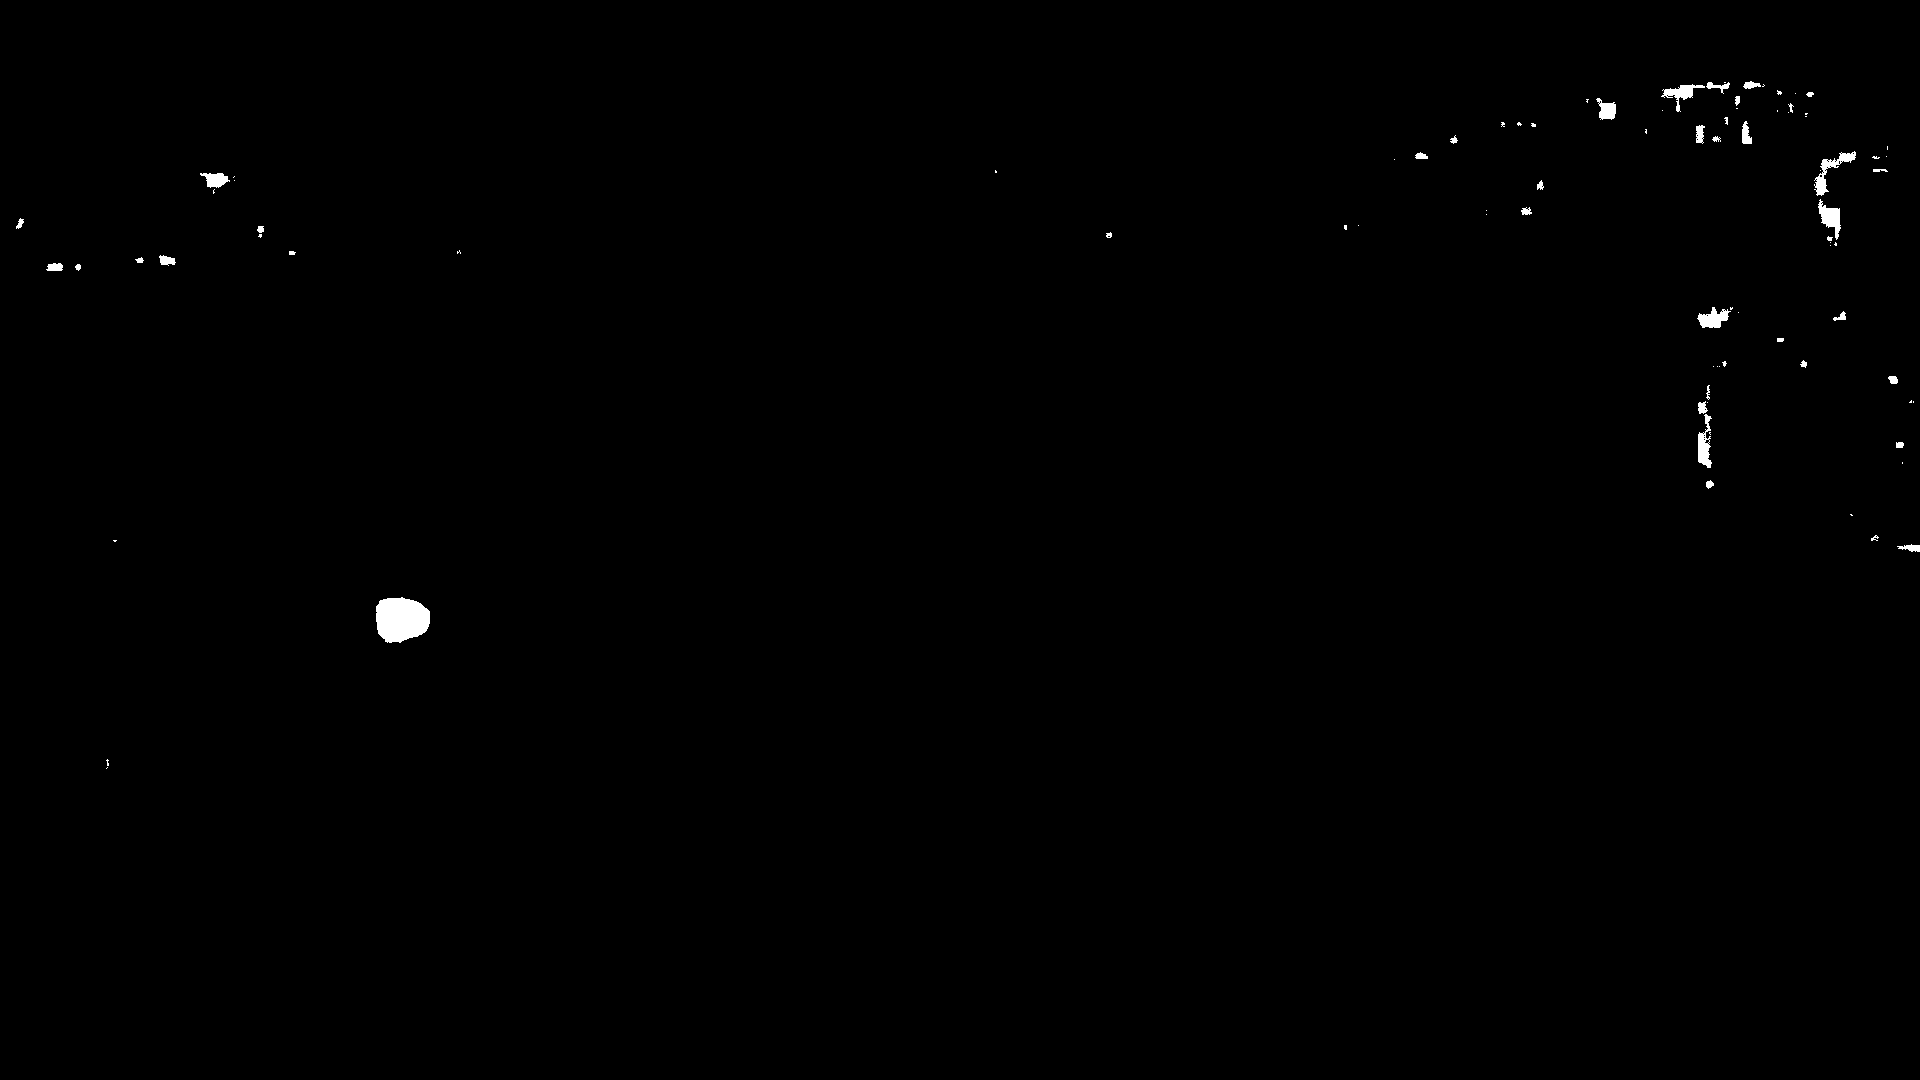
\includegraphics[width=\textwidth]{figures/frames/mask_131.png}}

        \end{minipage}
        \hfill
        \begin{minipage}{0.45\textwidth}
            \centering
            \subfloat[]{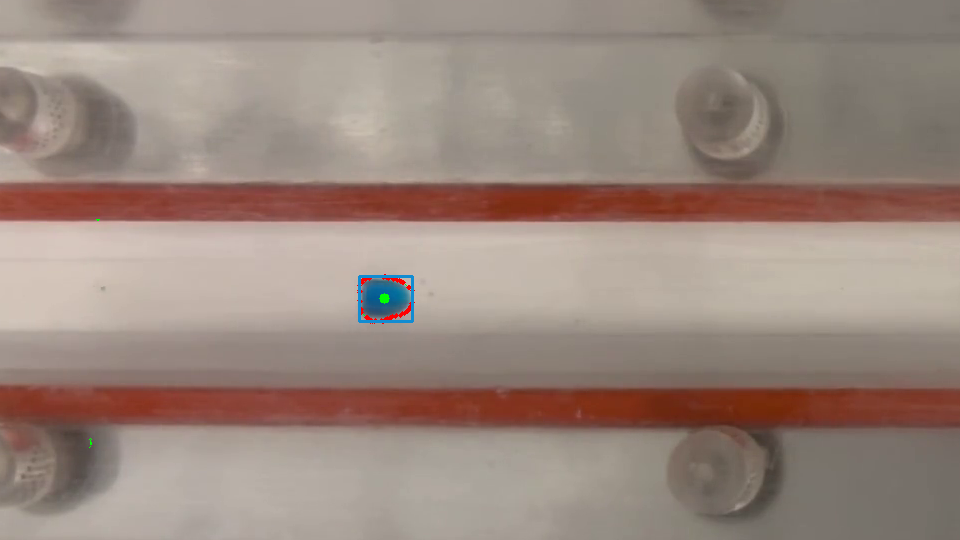
\includegraphics[width=\textwidth]{figures/frames/frame_131.png}}
        \end{minipage}
        \caption{Implementation of the computer vision algorithm. The frames show (a) a video frame with the droplet, (b) the color mask, and (c) the contour and bounds generated by the algorithm}
        \label{fig:CV_algorithm}
    \end{figure}

  \end{block}

  \begin{block}{Results: Initial Experimental Results}
    % Position vs time
      \begin{figure}
      \centering
      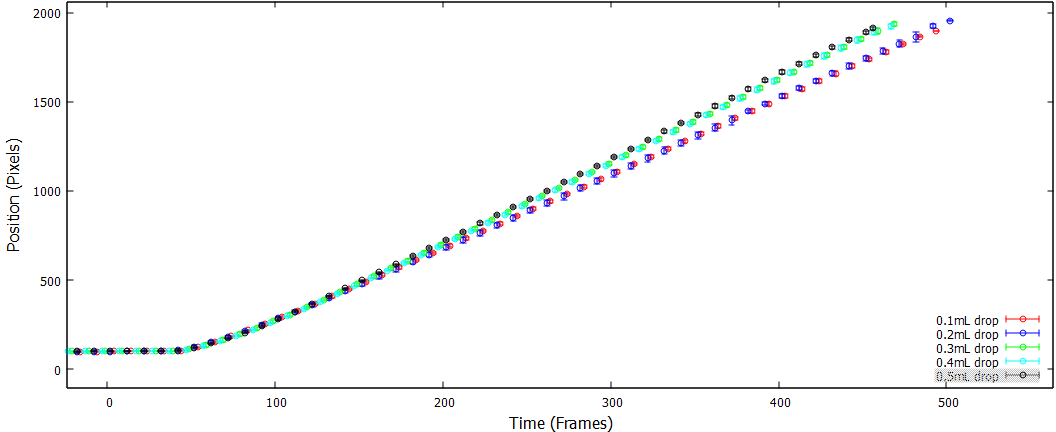
\includegraphics[width=0.55\linewidth]{figures/experimental_results/position time 15ml_min.png}
      \caption{Droplet position over time for 15mL/min bulk flow (normalized so that droplet motion starts at same frame)}
    \end{figure}
    % Taylor deformation vs time
    % \begin{figure}
    %   \centering
    %   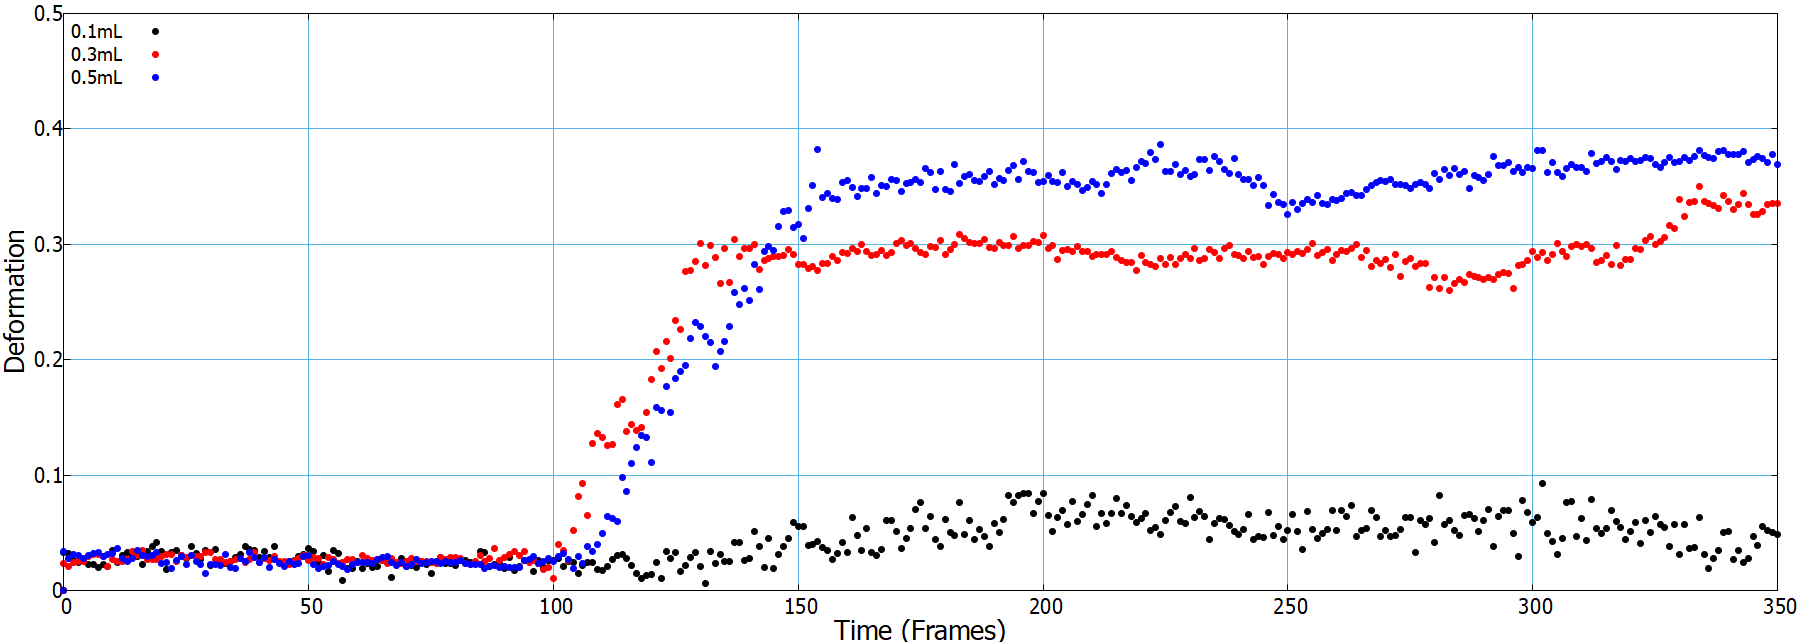
\includegraphics[width=0.65\linewidth]{figures/experimental_results/deformation time 15ml_min.png}
    %   \caption{Droplet Taylor deformation parameter over time for 15mL/min bulk flow}
    % \end{figure}
    \begin{figure}
        \centering
        \begin{minipage}{0.6\textwidth}
            \centering
            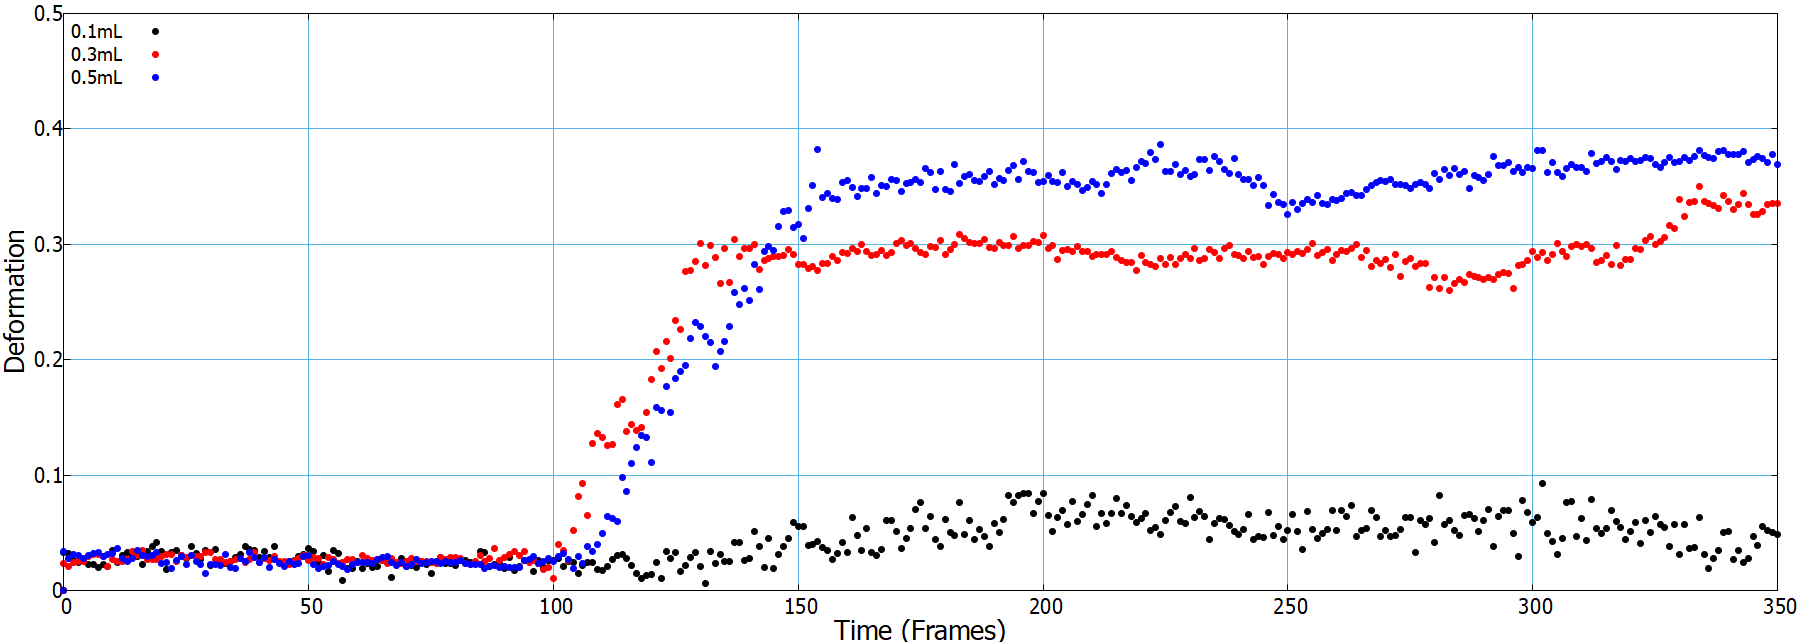
\includegraphics[width=\linewidth]{figures/experimental_results/deformation time 15ml_min.png}

        \end{minipage}
        \hspace{0.1\textwidth}
        \vspace{-0.5cm}
        \begin{minipage}{0.2\textwidth}
            \centering
            \begin{align*}
                \small
                \centering
                D_T &= \frac{L_{maj} - L_{min}}{L_{maj} + L_{min}} \\ \\
                L_{maj} &= \text{major semiaxis} \\ 
                L_{min} &= \text{minor semiaxis}
            \end{align*}
            \normalsize
        \end{minipage}
        \caption{Droplet Taylor deformation parameter over time for 15mL/min bulk flow (0.1, \textcolor{red}{0.3} and \textcolor{blue}{0.5} [mL])}
        \label{fig:TaylorDeformation}
    \end{figure}

  %   % avg velocities for different drop sizes
  %   \begin{figure}
  %     \centering
  %     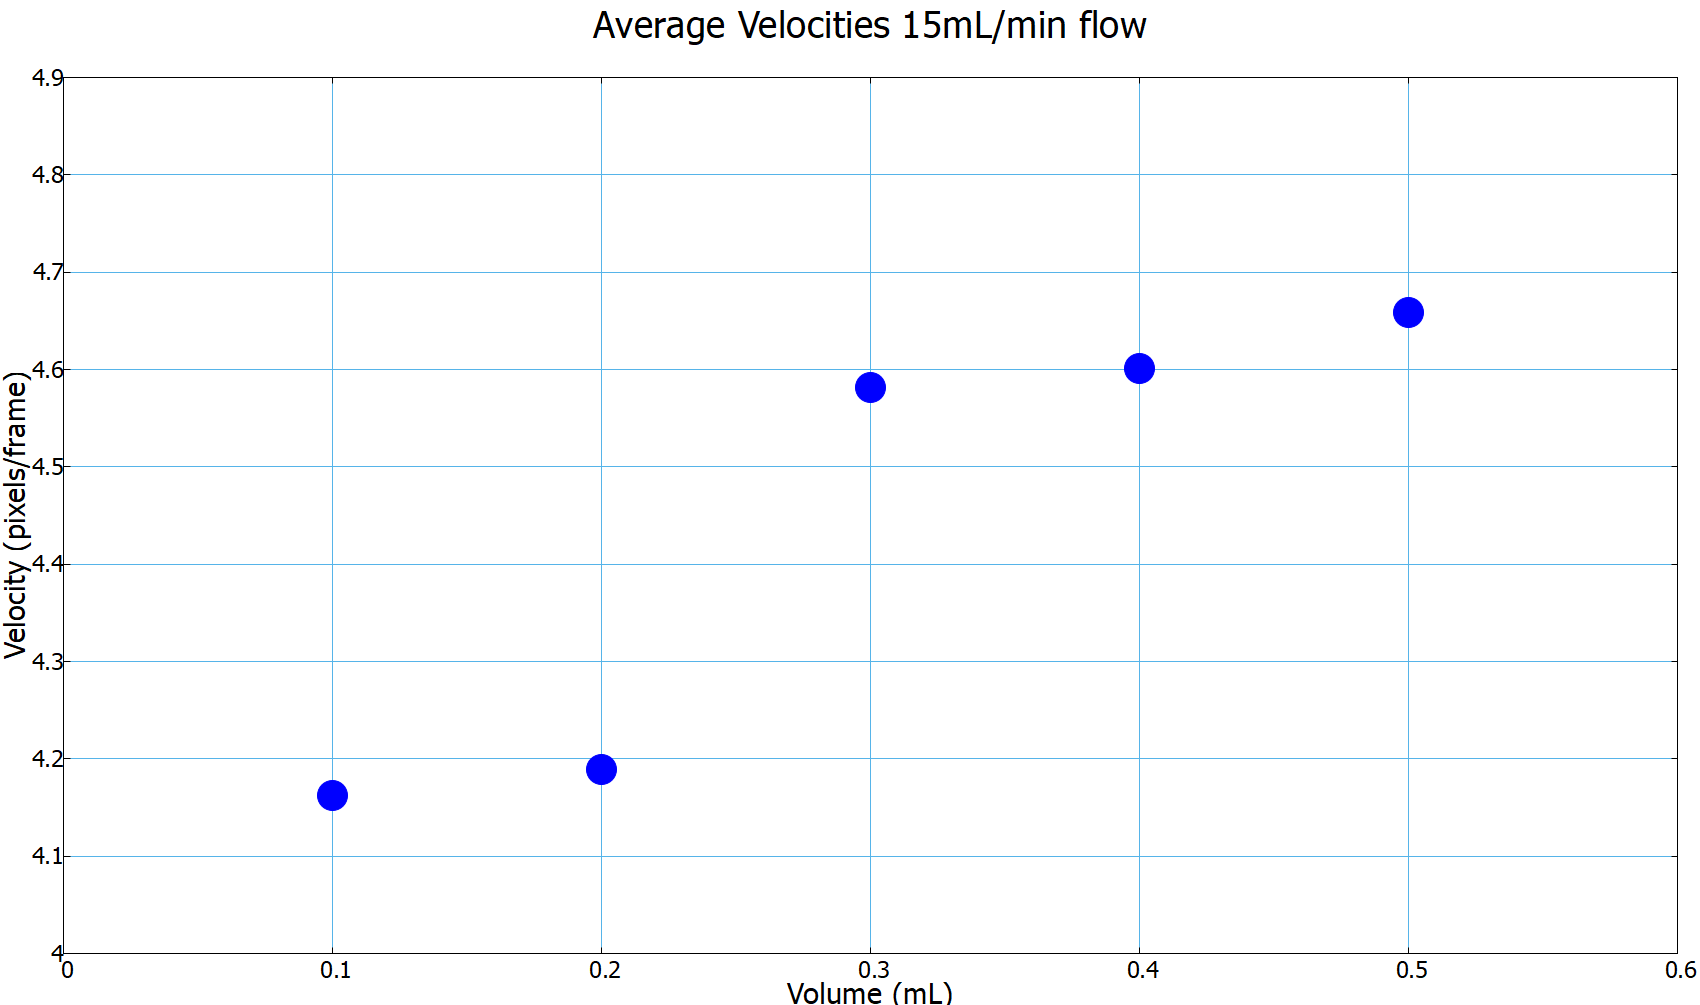
\includegraphics[width=0.65\linewidth]{figures/experimental_results/avg velocities drop sizes 15ml_min.png}
  %     \caption{Average velocity for different drop sizes with 15ml/min bulk flow}
  %   \end{figure}
  \end{block}

\end{column}

\separatorcolumn

\begin{column}{\colwidth}

  \begin{block}{Pendant Drop Experiments}
    
    \begin{columns}
        \begin{column}{.25\textwidth} % Left column and width
            \begin{figure}
                \centering
                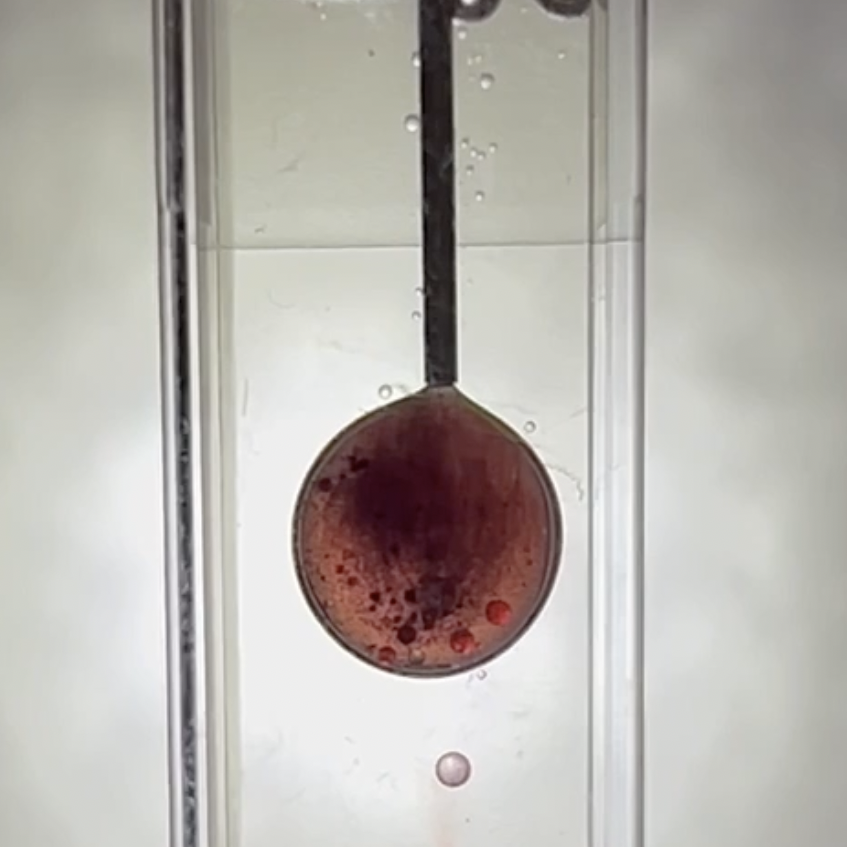
\includegraphics[width=\linewidth]{figures/pendantdrop.png}
                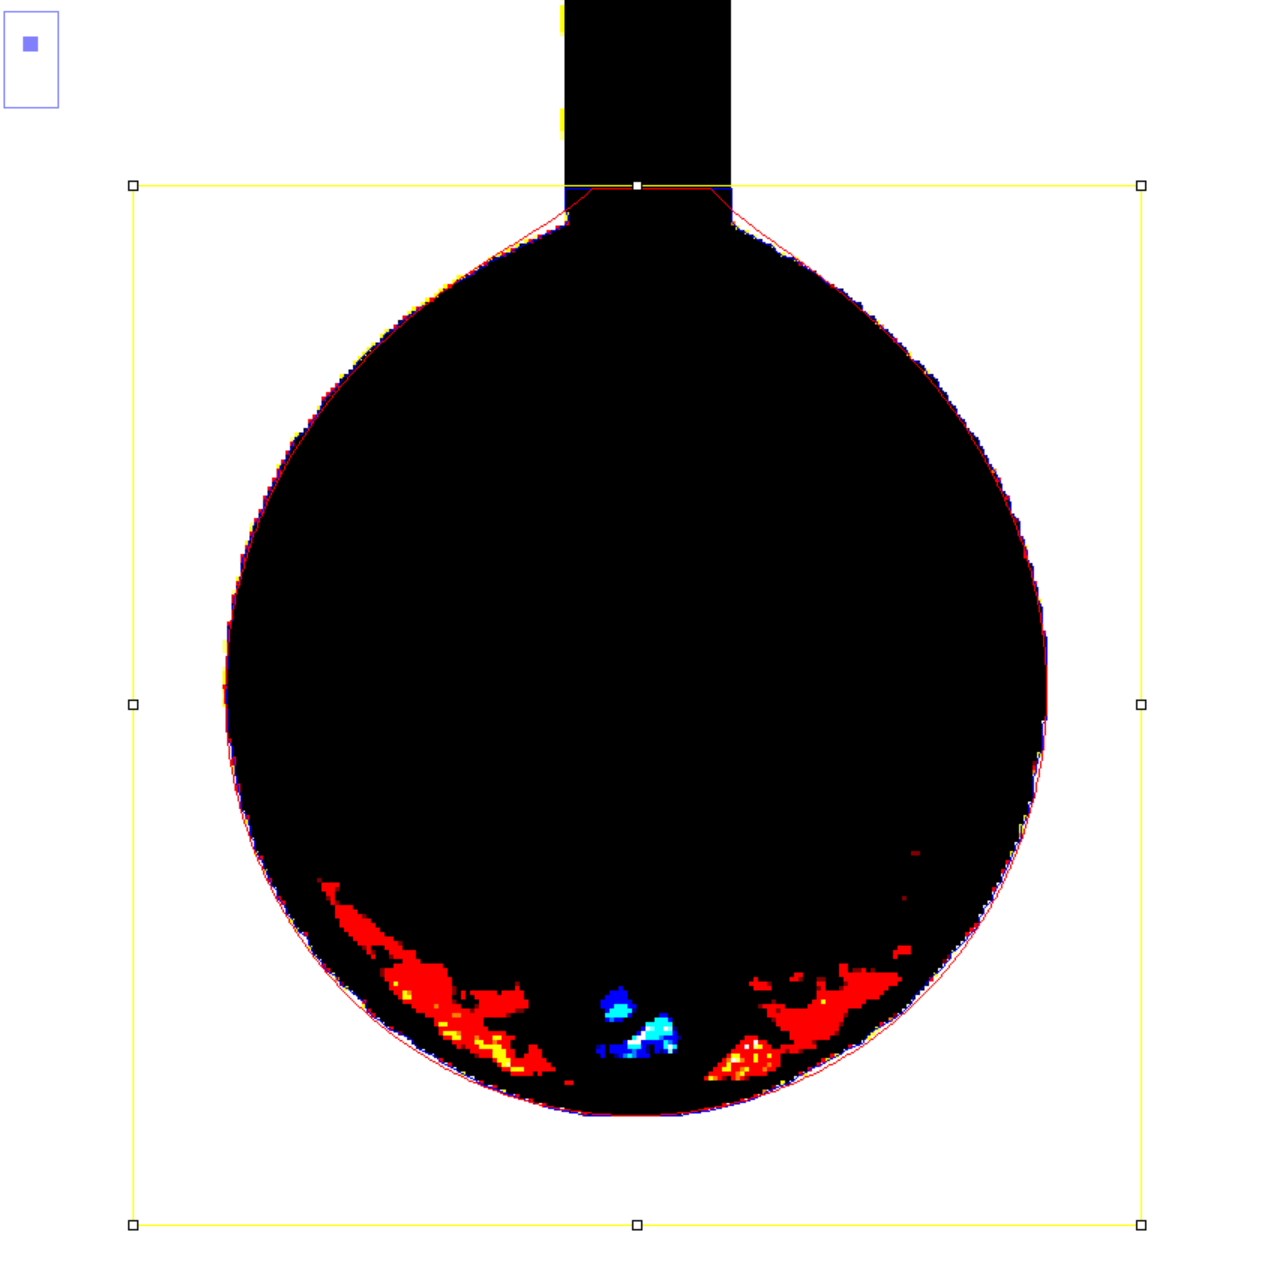
\includegraphics[width=\linewidth]{figures/binarization.png}
                \caption{Single frame of pendant drop experiment video and binarization from FIJI}
            \end{figure}
        \end{column}

        \begin{column}{.7 \textwidth} % Right column and width
            % Pendant drop schema
            \begin{figure}
                \centering
                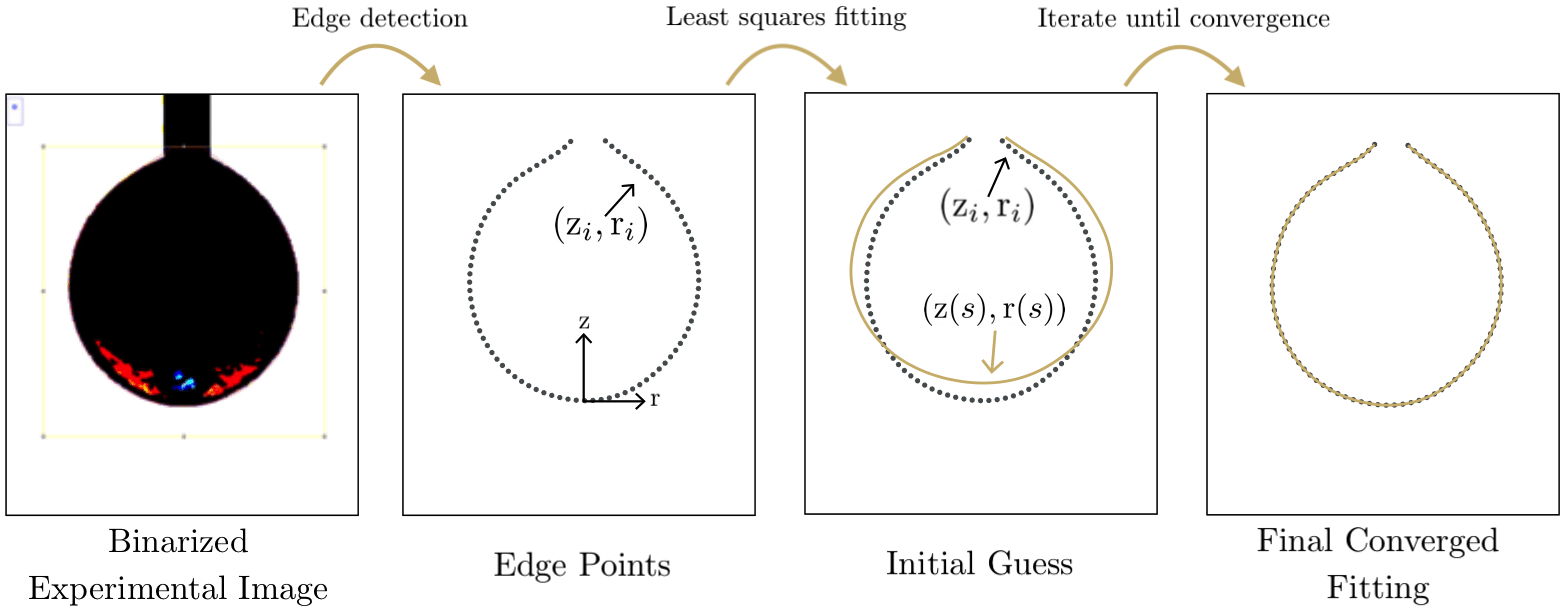
\includegraphics[width=\linewidth]{figures/Ashish_ExperimentFigure.png}
                \caption{Outline of the drop tensiometry process, adapted from \cite{berry_measurement_2015}}
            \end{figure}

            % Tabulate fluids
            \begin{table}
              \centering
              \begin{tabular}{l l c r}
                \toprule
                \textbf{Drop Phase} & \textbf{Bulk Phase} & \textbf{$\sigma \. \left[\frac{\text{mN}}{\text{m}}\right]$} & \textbf{Uncertainty} \\
                \midrule
                Water & Air & 77.7 & $\pm 5.8$ \\
                PDMS & Air & 22.5 & $\pm 3.3$ \\
                PDMS & Castor Oil & 18.0 & $\pm 3.1$ \\
                \bottomrule
              \end{tabular}
              \caption{Initial interfacial and surface tension values}
            \end{table}

            % Discuss results with water
            \centering
            Water has a tabulated $\sigma = 72 \frac{\text{mN}}{\text{m}}$
        \end{column}
    \end{columns}
    

  \end{block}
        
    \begin{exampleblock}{Concluding Remarks}
        \begin{itemize}
            \item Boundary integral method is efficient in simulating viscous droplets flowing in straight microchannels
            \item As $\lambda \nearrow$, deformation $\nearrow$ and $U_{av, ss} \searrow$ (more resistance to flow + high viscous stress)
            \item As $Ca \nearrow$, deformation $\nearrow$ and $U_{av, ss} \nearrow$ (more hydrodynamic shape)
            \item Good qualitative agreement between simulations and experiments, and promising interfacial tension results
        \end{itemize}
    \end{exampleblock}

    \begin{block}{Future Plans}
        \begin{itemize}
            \item FIJI $\rightarrow$ In-house code
            \begin{itemize}
                \item Lens distortion correction for experimental videos
                \item Isometric simulation videos
            \end{itemize}
            \item Determine interfacial tension values of droplet fluids
            \begin{itemize}
                \item In-house fitting code
            \end{itemize}
            \item Simulate droplets with experimentally determined conditions
            \item Improve regularity and control in apparatus
            \begin{itemize}
                \item Droplet origin and volume
            \end{itemize}
            \item \textbf{Maybe?} $\rightarrow$ PDMS microfluidic chip (Ding lab in Mechanical Engineering)
        \end{itemize}
    \end{block}

    \begin{block}{Acknowledgements}
    This body of work was made possible thanks to the support of
    \begin{itemize}
        \item Dr. Robert H. Davis, Tisone Professor and Dean Emeritus
        \item Gesse A. Roure, Ph.D. Candidate in Chemical and Biological Engineering
        \item Dr. Alexander A. Zinchenko, Senior Research Associate in the Davis Group
        \item Aditya V. Vepa and Adler Palos, Undergraduate researchers
        \item Isha Daukia and David Saeb, Assistance with figures
    \end{itemize}
    \end{block}

    \begin{block}{References}
        \small
        \begin{thebibliography}{9}
            \bibitem{navarro_boundary-integral_2020}
            Navarro, R. and Zinchenko, A.Z. and Davis, R.H.
            \newblock Boundary-integral study of a freely suspended drop in a {T}-shaped microchannel.
            \newblock {\em International Journal of Multiphase Flow}, 130:103379, September 2020.

            \bibitem{Roure_2022}
            Roure, G. A., and Zinchenko A.Z., and Davis, R. H.
            \newblock Numerical Simulation of Deformable Droplets in Complex-Shaped Microchannels.
            \newblock {\em (to be submitted)}.
            
            % \bibitem{zinchenko_novel_1997}
            % Zinchenko, Alexander Z. and Rother, Michael A. and Davis, Robert H.
            % \newblock A novel boundary-integral algorithm for viscous interaction of deformable drops.
            % \newblock {\em Physics of Fluids}, 9(6):1493--1511, June 1997.
            
            \bibitem{zhang_flexible_2000}
            Zhang, Z.
            \newblock A flexible new technique for camera calibration.
            \newblock {\em IEEE Transactions on Pattern Analysis and Machine Intelligence}, 22(11):1330--1334, November 2000.
            
            \bibitem{berry_measurement_2015}
            Berry, J.D. and Neeson, M.J. and Dagastine, R.R. and Chan, D.Y.C. and Tabor, R.F.
            \newblock Measurement of surface and interfacial tension using pendant drop tensiometry.
            \newblock {\em Journal of Colloid and Interface Science}, 454:226--237, September 2015.
            

        \end{thebibliography}
        \normalsize
    
        % if using bibtex
        % \nocite{*}
        % \footnotesize{\bibliographystyle{plainnat}\bibliography{poster}}

    \end{block}

\end{column}

\separatorcolumn
\end{columns}
\end{frame}

\end{document}